
% Works
% -----

\subsection{Domains of Sets and Inverse Sequences}

\begin{mydef}[Sets of sequences]
As we will frequently refer to sets of fequences,
we will use calligraphic letters (e.g. $\sqs{A}$, $\sqs{B}$, $\sqs{C}$ and $\sqs{S}$)
to denote such sets for brevity.

We will write $\Dom{\sqs{A}}$ for $\bigcap_{A\in\sqs{A}} \Dom{A}$,
and $\sqs{A}\cc\sqs{B}$ for $\{A\cc B\whr A\in\sqs{A}, B\in\sqs{B}\}$.

% This has only been defined for sequences, not sets.
Moreover, we write $\wrks{\sqs{A}}$ if $\varnothing \subset \Dom{\sqs{A}}$, that is,
if we know that there is at least one filesystem
all sequences in $\sqs{A}$ are defined on.
\end{mydef}

% works operators
% ---------------

\begin{mydef}[$\worksmeqsign$]\label{def_works}
For two sets of sequences $\sqs{A}$ and $\sqs{B}$
we write $\worksm{\sqs{A}}{\sqs{B}}$ iff $\Dom{\sqs{A}} \subseteq \Dom{\sqs{B}}$;
that is, iff all sequences in $\sqs{B}$ are defined on (do not break)
all filesystems on which sequences in $\sqs{A}$ are defined.
\end{mydef}

When $\sqs{A}$ or $\sqs{B}$ contains a single sequence,
we leave out the curly brackets and write,
e.g. $A\cc\sqs{B}$ to mean $\{A\}\cc\sqs{B}$,
or $\worksm{A}{B}$ to mean $\worksmbb{A}{B}$.

We can see that $A\eqext B$ implies $\worksm{A}{B}$, as the latter
only requires that $B$ is defined where $A$ is defined, 
while the former also requires
that where they are defined, their effect is the same.

The following claim follows immediately from the definition:

\begin{myclm}\label{worksextpostfix}
% An inference rule in the algebra
$\forall A,S: \worksm{A\cc S}{A}$, that is, if a sequence is defined,
its initial segments are also defined.
\end{myclm}

We also prove the following lemmas.

\begin{myax}\label{combine_independent_commands}
The combination of independent commands is defined on all filesystems
where both of the commands are defined:
\[ \alpha\indep \beta \Rightarrow \worksmbx{\alpha, \beta}{\alpha\cc \beta}. \]
\end{myax}
\begin{proof}
We name this proposition a \namecref{combine_independent_commands} 
because to prove it, we must reach back to our filesystem model.
Let $\alpha=\cxynv$ and $\beta=\czwmv$.
The proof is by contradiction;
assume that there is a filesystem $\FS$ for which
$\cxynv\aFS\neq\fsbroken$ and $\czwmv\aFS\neq\fsbroken$, but
$\cxynv\cc \czwmv\aFS=\fsbroken$.
We know $\cxynv\aFS\neq\fsbroken$ so it must be applying 
$\czwmv$ that breaks it.
Applying a command can only result in a broken filesystem in two cases.
First, if the input type does not match the filesystem,
but we know $[\FS(m)]=[w]$ and so
$[(\cxynv\aFS)(m)]=[w]$ as based on \cref{incomparable_is_independent}, $n\neq m$.
Second, if the new filesystem violates the tree property.
This again cannot be the case because we also know that $n\unrel m$
and the tree property only depends on the types of values at the parent and children of $m$,
which therefore cannot be changed by $\cxynv$.
\end{proof}

\cref{combine_independent_commands} extends to sequences as well:

\begin{mylem}\label{combine_independent_sequences}
The combination of independent sequences is defined on all filesystems
where both of the sequences are defined:
\[ S\indep T \Rightarrow \worksmbx{S,T}{S\cc T}. \]
\end{mylem}
\begin{proof}
Assume that there is a filesystem $\FS$ so that
$S\aFS\neq\fsbroken$ and $T\aFS\neq\fsbroken$, but
$(S\cc T)\FS=\fsbroken$.

From \cref{def_indep} we know that
the commands in $S$ and $T$ pairwise commute, and so any sequence
that contains the commands from $S$ and $T$ and preserve their original partial order
is equivalent to $S\cc T$ on all filesystems.

Let the command in $T$ that breaks $\FS$ when applying $S\cc T$ be $t$
so that $T=T_0\cc t\cc T_1$.
It is still true that $(T_0 \cc t)\FS\neq\fsbroken$,
and by definition $(S\cc T_0)\FS\neq\fsbroken$,
but $(S\cc T_0\cc t)\FS=\fsbroken$.
Also, from above we know that $S\cc T_0\equiv T_0\cc S$
and so $(T_0 \cc S)\FS\neq\fsbroken$.

If we denote the first command in $S$ with $s_1$,
this means that $(T_0 \cc s_1)\FS\neq\fsbroken$,
which we can combine with $(T_0 \cc t)\FS\neq\fsbroken$, $t\indep s_1$ and
\cref{combine_independent_commands}
(using $T_0\FS$ as the reference filesystem)
to arrive at $(T_0 \cc s_1\cc t)\FS\neq\fsbroken$.

We can repeat this step for $s_2$, the next command in $S$,
and from 
$(T_0 \cc s_1\cc t)\FS\neq\fsbroken$
and
$(T_0 \cc s_1\cc s_2)\FS\neq\fsbroken$
arrive at
$(T_0 \cc s_1\cc s_2\cc t)\FS\neq\fsbroken$.
This can be repeated until $S$ is exhausted and we get
$(T_0 \cc S\cc t)\FS\neq\fsbroken$, which is a contradiction.
\end{proof}

We also prove the following:

\begin{mylem}\label{worksinputmatch}
If $S$ and $T$ are minimal sequences, $\worksmnilb{S,T}$,
and there are commands on node $n$ in both $S$ ($\cxynv\in A$) and $T$ ($\czwnv\in B$),
then the input types of these commands must match, i.e. $[x]=[z]$.
\end{mylem}
\begin{proof}
This result is similar to \cref{equiv_simple_same_commands} and
is easily shown using a proof by contradiction: if $[x]\neq [z]$, then there is no filesystem that
either $\cxynv$ or $\czwnv$ would not break, 
and consequently $S$ and $T$ cannot work on the same filesystem.
\end{proof}


\bigskip

% Type equivalence classes
% ------------------------

\noindent
For the proof of the correctness of the reconciliation algorithm,
we will also need a way of moving parts of sequences between the two
sides of the $\worksmeqsign$ relation.
We can do this based on the observation that commands are bijections
if we only distinguish between types in our objects.
To formalise this, we extend type equality ($\typeeq$)
to filesystems, commands and sequences of commands.
\begin{mydef}[Equivalence by type, extended: $\typeeq$]
$ $ % otherwise first list element starts on same line
\begin{itemize}
\item For two filesystems in $\setfs$, $\FS\typeeq\GS$ iff
for all $n\in\setn$, $\FS(n) \typeeq \GS(n)$.
\item For two commands $\cxynv\typeeq\czwmv$ iff 
$x\typeeq z$ and $y\typeeq w$
(that is, $[x]=[z]$ and $[y]=[w]$)
and $n=m$.
\item To sequences of commands, the relation $\typeeq$ extends as usual: $\emptyseq\typeeq\emptyseq$, and
if $A'=\alpha\cc A$ and $B'=\beta\cc B$, then $A'\typeeq B'$ iff $\alpha\typeeq\beta$ and $A\typeeq B$.
\end{itemize}
\end{mydef}

We select representatives from each $\typeeq$-equivalence class of values:
for $[\empt]$ and $[\vald]$ this must be $\empt$ and $\vald$; and
for $[\valf]$ we select an arbitrary file value $\fil\in[\valf]$.
We then use these representative values to
introduce the \emph{canonical mapping} $\T{}$ that preserves the types of values,
but maps all objects into a subsystem where there is a one-to-one
correspondence between types and values.

\begin{mydef}[canonical mapping, $\T{}$]\label{def_typemapping}
We use $\T{}$ and write $\T{a}$ to denote the canonical mapping of 
values, filesystems, commands and sequences to the
representatives of their $\typeeq$-equivalence class.
\begin{itemize}
\item For values, $\T{\vald}=\vald$, $\T{\valf}=\fil$ and $\T{\empt}=\empt$.
\item For filesystems, $\T{\FS}$ is defined by $\T{\FS}(n) = \T{\FS(n)}$.
\item For commands, $\T{\cbrk}=\cbrk$ and $\T{\cxynv} = \cTxynv$.
\item To sequences of commands, the mapping extends as usual: $\T{\emptyseq}=\emptyseq$, and if $S'=\alpha\cc S$, then $\T{S'}=\T{\alpha}\cc \TS$.
\item Finally we extend $\T{}$ to sets of sequences: $\T{\sqs{A}} = \{\TS \whr S\in\sqs{A}\}$.
\end{itemize}
\end{mydef}

We refer to any object in the image of $\T{}$ as \emph{canonical}.

By definiton,
for any filesystem $\FS$ and command $\alpha$, 
$\T{\alpha}(\T{\FS}) = \T{(\alpha\aFS)}$.


% TODO ???
Also, for all objects where it is defined, $\T{a}\typeeq a$.
As canonical filesystems, commands, sequences, etc.
are subsets of their non-canonical counterparts, 
all propositions proven so far apply to them as well.


As the types of values determine whether a command breaks a filesystem,
we know $\Dom{A}=\Dom{\TA}$ and therefore $\Dom{\sqs{A}}=\Dom{\T{\sqs{A}}}$.
From this it follows that
% TODO what's the set of all filesystems?
% TODO:
\begin{mycor}\label{repr_works_is_same}
\begin{gather*}
\worksmnil{\sqs{A}} \Longleftrightarrow \worksmnil{\T{\sqs{A}}} \\
\worksm{\sqs{A}}{\sqs{B}} \Longleftrightarrow \worksm{\T{\sqs{A}}}{\T{\sqs{B}}}.
\end{gather*}
\end{mycor}

% Inverse commands
% ----------------

We are now ready to define the inverse of canonical commands $\T{\alpha}$
which allows us to move parts of sequences between the
two sides of $\worksmeqsign$.
This is based on the following observation.

% TODO \alpha \neq \cbrk
\begin{mylem}\label{repr_comm_inject}
Canonical commands $\T{\alpha}$ are partial bijections over canonical filesystems
($\T{\FS}$, $\T{\GS}$).
Because partial functions are trivially surjective when restricted to their images, this is
equivalent to saying that canonical functions are injective except for cases
where they are not defined:
\begin{align*}
\forall\FS,\GS,\alpha:& \\
& \T{\FS}\neq\T{\GS} \wedge \T{\alpha}(\T{\FS})\neq\fsbroken \\
& \Rightarrow \T{\alpha}(\T{\FS}) \neq \T{\alpha}(\T{\GS}).
\end{align*}
\end{mylem}
\begin{proof}
Choose values that satisfy the left side, and let $\T{\alpha} = \cTxynv$.
If $\T{\FS}$ and $\T{\GS}$ have different values (types) at any node apart from $n$, then this difference remains
even after applying $\cTxynv$ to $\T{\FS}$. 
The only remaining case therefore is where they have the same values
at all nodes except at $n$.
As $\cTxynv(\T{\FS})\neq\fsbroken$, we know $[\FS(n)]=[x]$.
We also know that $\T{\GS}(n)\neq\T{\FS}(n)$, and therefore
$[\GS(n)]\neq[x]$.
This implies $\cTxynv(\T{\GS})=\fsbroken$,
and again we have $\T{\alpha}(\T{\FS}) \neq \T{\alpha}(\T{\GS})$.
\end{proof}

% See
% https://en.wikipedia.org/wiki/Inverse_semigroup#Origins
% https://en.wikipedia.org/wiki/Symmetric_inverse_semigroup
% https://en.wikipedia.org/wiki/Partial_function

\begin{mydef}[Inverse commands and sequences]
We write $\T{\alpha}^{-1}$ for
the inverse of the canonical command (partial bijection) $\T{\alpha}$,
which is uniquely defined by \cref{repr_comm_inject}.

We write $\TS^{-1}$ for the inverse of the sequence $\TS$, which consists of the inverses of the commands in $\TS$ in reverse order.
\end{mydef}
By definition, for any canonical filesystem $\T{\FS}$ outside the image of 
$\T{\alpha}$, the inverse $\T{\alpha}^{-1}$ is not defined.

% Some further observations:
% For canonical commands \[ \cTxynv^{-1} = \cTyxnv. \]
% $\forall S: ({\TS}^{-1})^{-1} = \TS$.

For brevity, in the following lemma we use $B$, $B'$, $\sqs{A}$ and $\sqs{C}$ to denote
canonical sequences and sets.

\newcommand{\ia}{\sqs{A}}
\newcommand{\ic}{\sqs{C}}
\newcommand{\ibi}{B^{-1}}

\begin{mylem}\label{r_invmove}
A common initial segment of a set of canonical sequences can be moved 
to the other side of $\worksmeqsign$ by inverting it:
\begin{gather*}
\worksm{\ia}{B\cc\ic}
\ \Longleftrightarrow \ \worksm{\ibi\cc\ia}{\ic} 
\ \wedge \  \worksm{\ia}{\{B\}}
\end{gather*}
\end{mylem}
\begin{proof}
% This result is quite expected as we're mapping a subset statement using a bijection,
% but made more complicated a as B is not defined everywhere.

The proof is illustrated by \cref{fig_invmove}.

\begin{figure}[htb]
\begin{center}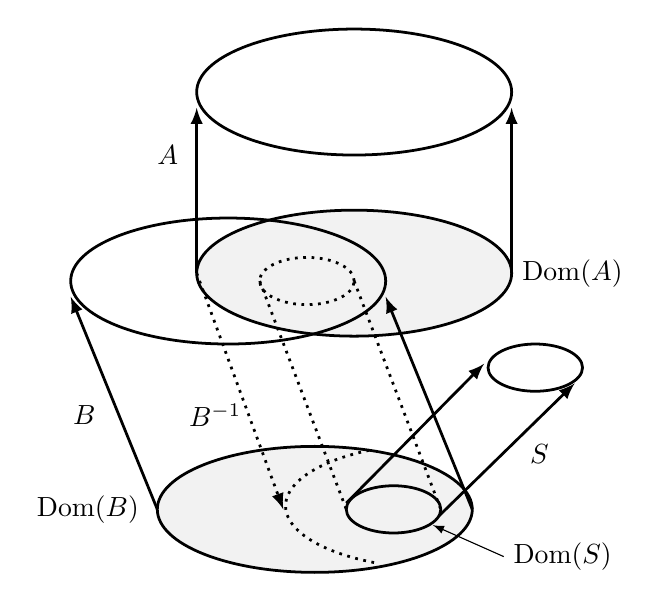
\begin{tikzpicture}
[line width=1pt]
\node at  (1.6+2, 0.1) [right] {$\textrm{Dom}(\seqset{A})$};
\draw[fill=black!5] (1.6, 0.1) ellipse (2cm and 0.8cm); %% Dom A
\draw               (1.6, 2.4) ellipse (2cm and 0.8cm); %% Img A
\draw[-latex] (1.6+2, 0.1)--(1.6+2, 2.4-.2); %% A right
\draw[-latex] (1.6-2, 0.1)--(1.6-2, 2.4-.2); %% A left
\node at  (1.6-2-.1, 1.6) [left] {$A$};
%%
\node at (1.1-2-.1, -2.9) [left] {$\textrm{Dom}(B)$};
\draw[fill=black!5] (1.1, -2.9) ellipse (2cm and 0.8cm); %% Dom B
\draw               (0  ,  0)   ellipse (2cm and 0.8cm); %% Img B
\draw[-latex] (1.1+2, -2.9)--(0+2, 0-.2); %% B right
\draw[-latex] (1.1-2, -2.9)--(0-2, 0-.2); %% B left
\node at  (0.55-2-.1, -1.7) [left] {$B$};
\draw[-latex,dotted] (1.6-2, 0.1)--(0.7, -2.9); %% B-1
\node at (0.3, -1.7) [left] {$B^{-1}$};
\draw[dotted] (1.79, -2.15) arc(118:244: 2cm and 0.8cm); %% Arc
\draw[dotted] (1, 0) ellipse (0.6cm and 0.3cm); %% Dotted S
\draw         (2.1, -2.9) ellipse (0.6cm and 0.3cm); %% Dom S
\draw[dotted] (1-0.6, 0)--(2.1-0.6, -2.9); %% B-1
\draw[dotted] (1+0.6, 0)--(2.1+0.6, -2.9); %% B-1
\draw                     (3.9, -1.1) ellipse (0.6cm and 0.3cm); %% Img S
\draw[-latex] (2.1-0.6, -2.9+.08)    --(3.9-0.6-.05, -1.1+.05); %% Left S
\draw[-latex] (2.1+0.6-.02, -2.9-.08)--(3.9+0.6-.1, -1.1-.2); %% Right S
\node at  (3.7,-2.2) [right] {$S$};
\draw[-latex,thin] (3.5, -3.5) node[right]{$\mathrm{Dom}(\seqset{S})$} -- (2.1+0.5, -2.9-0.2);
\end{tikzpicture}\end{center}

\caption{Proof of \cref{r_invmove}}\label{fig_invmove}
\end{figure}

For the left-to-right part of the proposition,
from $\worksm{\ia}{B\cc\ic}$ we know $\Dom{\ia} \subseteq \Dom{B\cc\ic}$.
As the (canonical) $B$ is a bijection between its domain and image,
we can use $B$ to map both sides of this statement, which yields
$\Dom{B^{-1}\cc\ia} \subseteq \Dom{\ibi\cc B\cc\ic}$,
but the latter is a subset of $\Dom{\ic}$,
and so $\Dom{\ibi\cc\ia} \subseteq \Dom{\ic}$,
which means that $\worksm{\ibi\cc\ia}{\ic}$.
It is easy to see that $\worksm{\ia}{B\cc\ic} \Rightarrow \worksm{\ia}{B}$.

For the right-to-left part,
from $\worksm{\ia}{B}$ we know $\Dom{\ia} \subseteq \Dom{B}$.
Therefore we can project the whole of $\Dom{\ia}$ using the bijective canonical sequence $B$
to get $\Dom{\ibi\cc\ia}$, and as $\worksm{\ibi\cc\ia}{\ic}$
we know
$\Dom{\ibi\cc\ia} \subseteq \Dom{\ic}$.
We use $\ibi$ to project both sides of this statement to get
$\Dom{B\cc\ibi\cc\ia} \subseteq \Dom{B\cc\ic}$.
But we also know that $\Dom{B\cc\ibi\cc\ia} = \Dom{\ia}$
as $\Dom{\ia} \subseteq \Dom{B}$,
and so $\Dom{\ia} \subseteq \Dom{B\cc\ic}$ which means
$\worksm{\ia}{B\cc\ic}$.
\end{proof}

We use this result to prove the following:

\begin{mylem}\label{indep_prefix_combine}
The combination of two sequences with a common head and independent tails 
is defined wherever the two sequences are defined:
\[ B\indep C \Rightarrow \worksmbx{A\cc B, A\cc C}{A\cc B\cc C} \]
\end{mylem}
\begin{proof}
This is trivial unless $\worksmnil{A}$, so we assume that that is the case.
From $B\indep C$ and \cref{combine_independent_sequences} we know
$\worksmbx{B, C}{B\cc C}$.
Based on \cref{repr_works_is_same} this is equivalent to
$\worksmbx{\TB, \TC}{\TB\cc \TC}$.
Since $\TA^{-1}\cc \TA \equiv \emptyseq$, this can also be written as
\[\worksm{\TA^{-1}\cc\{\TA\cc \TB, \TA\cc \TC\}}{\TB\cc \TC}.\]
From \cref{worksextpostfix} we also know that
$\worksmbx{\TA\cc \TB, \TA\cc \TC}{\TA}$.
Combining the last two statements using \cref{r_invmove}
we get
\[ \worksmbx{\TA\cc \TB, \TA\cc \TC}{\TA\cc \TB\cc \TC}, \]
which with \cref{repr_works_is_same} proves the
\namecref{indep_prefix_combine}.
\end{proof}
